\section{Predicción del Ganador}
Para la predicción del ganador hemos creado una interficie gráfica para poder dejar experimentar a aquel que quiera con los diferentes modelos. Para poder ejecutar esta interfaz, se tienen que cumplir todos los \texttt{requirements.txt} y más tarde dentro del \textit{PATH} ejecutar el siguiente comando \texttt{streamlit run presentation.py}. Esto nos abrirá en local una interficie gráfica con el siguiente formato.

\begin{figure}[H]
\centering
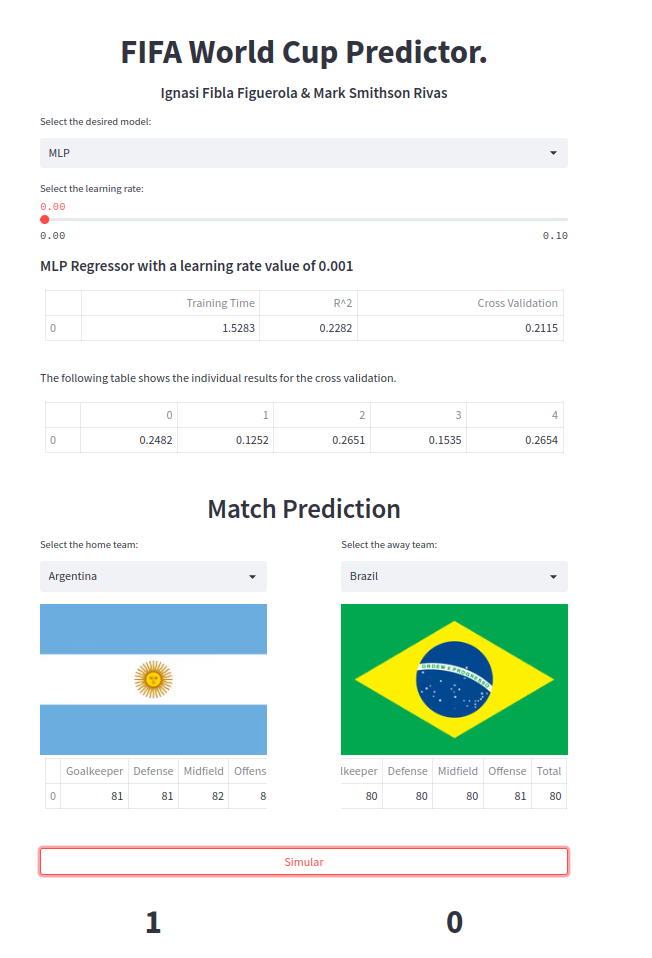
\includegraphics[width=10cm]{images/webPage.png}
\caption{Interficie Gráfica}
\label{Interficie-grafica}
\end{figure}

En esta interficie se pueden simular partidos con el modelo que el usuario desee y con los parámetros que se especifiquen.
\newline

Con esta herramienta hemos generado el resultado del mundial de Qatar de 2022, desde los cuartos de finales para no hacer tantos partidos. El modelo está forzando a que uno dé los dos equipos gane y los resultados están centrados en 0, es decir, un 1-0 significa que el local ha ganado por diferencia de 1 al visitante. Es importante también respetar quién es local y quién es visitante en cada partido, ya que esto afecta a la predicción.
\newline

Una vez predecidos los partidos hemos obtenido el siguiente resultado:

\begin{figure}[H]
\centering
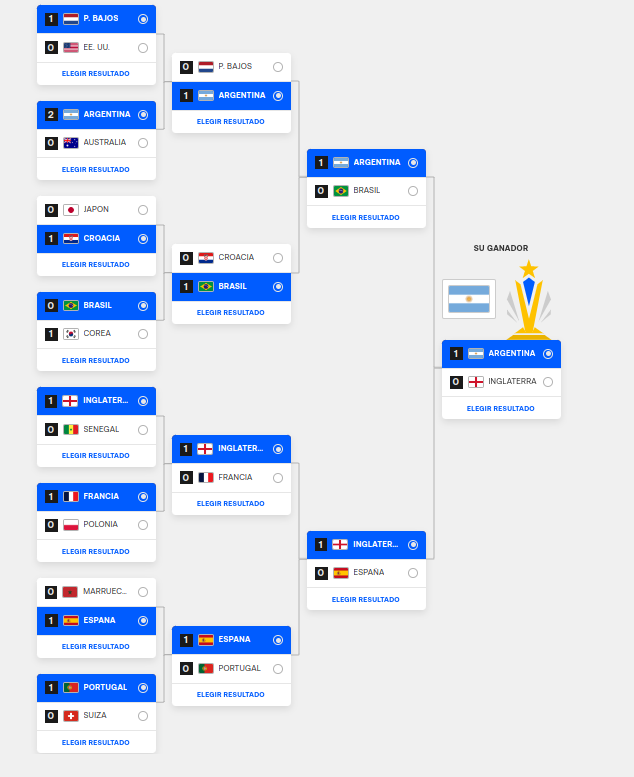
\includegraphics[width=12cm]{images/prediction.png}
\caption{Interficie Gráfica}
\label{Interficie-gráfica}
\end{figure}

Como podemos observar, nuestro modelo ha acertado la mayoría de los partidos pese a algunos que no, ya que dieron la sorpresa como Marruecos ganando a España o Croacia ganando a Brasil. Nuestro modelo predice que Argentina es campeona, tal y como pasó en la vida real, y predice una final de Argentina-Brasil, que muchos otros modelos y gente hablaba de que está sería la final.

\newpage